%% Beispiel-Präsentation mit LaTeX Beamer im KIT-Design
%% entsprechend den Gestaltungsrichtlinien vom 1. August 2020
%%
%% Siehe https://sdqweb.ipd.kit.edu/wiki/Dokumentvorlagen

%% Beispiel-Präsentation
\documentclass{sdqbeamer} 
 
%% Titelbild
\titleimage{banner_2020_kit (1)}

%% Gruppenlogo
\grouplogo{white_image.png} 

%% Gruppenname und Breite (Standard: 50 mm)
\groupname{KASTEL, DSiS}
%\groupnamewidth{50mm}

% Beginn der Präsentation

\title[Automatisiertes Testen von Programmiermethodik]{Automatisiertes Testen von
Programmiermethodik}
\subtitle{Ingenieursmäßige Softwareentwicklung} 
\author[David Laubenstein]{David Laubenstein}

\date[20.\,03.\,2023]{20. März 2023}

% Literatur 
 
\usepackage[citestyle=authoryear,bibstyle=numeric,hyperref,backend=biber]{biblatex}
\usepackage[inkscapeformat=png]{svg}
\addbibresource{presentation.bib}
\bibhang1em

\usepackage{listings}
\lstset{language=Java,
                basicstyle=\footnotesize\ttfamily,
                keywordstyle=\footnotesize\color{blue}\ttfamily,
}

\begin{document}
 
%Titelseite
\KITtitleframe

%Inhaltsverzeichnis
% sollte weg laut betreuern
% \begin{frame}{Inhaltsverzeichnis}
% \tableofcontents
% \end{frame}

\section{Motivation}
% Motivation -> es sind viele studenten (800 Abgaben fast), je mehr automatisiert, desto besser... 
\begin{frame}{Motivation: Aktueller Stand}
    \begin{columns}
        \begin{column}{0.48\textwidth}
            \begin{figure}
                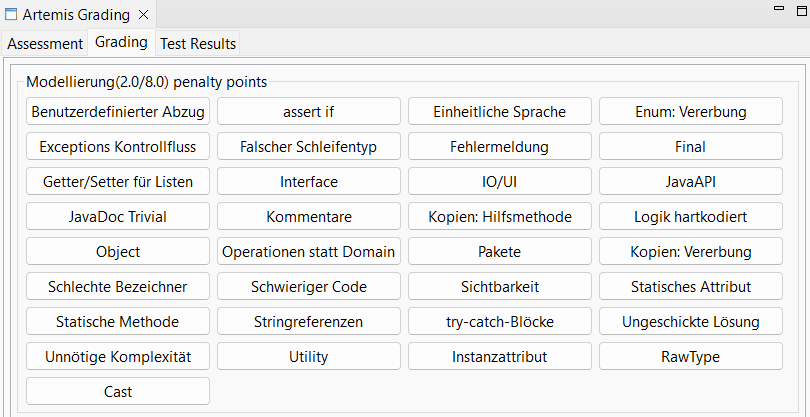
\includegraphics[scale=0.38]{logos/gradingedition_grading.png}
                \caption{\cite{gradingTool}}
                \label{fig:gradingTool}
            \end{figure}
        \end{column}
        \pause
        \begin{column}{0.48\textwidth}
            \begin{center}
            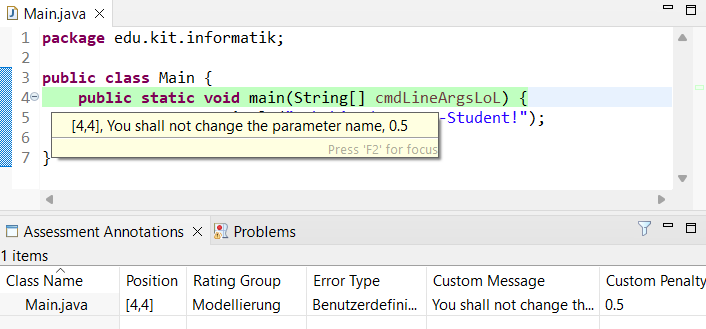
\includegraphics[scale=0.38]{logos/gradingedition_annotation.png}
            \end{center}
        \end{column}
    \end{columns}
\end{frame}

\begin{frame}{Motivation: Ziel}
    \begin{columns}
        \begin{column}{0.48\textwidth}
            \begin{figure}
                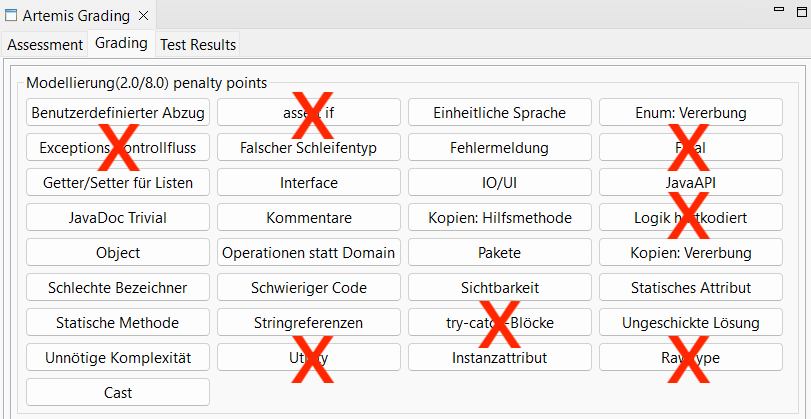
\includegraphics[scale=0.38]{logos/gradingedition_grading_done.png}
                \caption{\cite{gradingTool}}
                \label{fig:gradingTool}
            \end{figure}
        \end{column}
        \begin{column}{0.48\textwidth}
            \begin{center}
            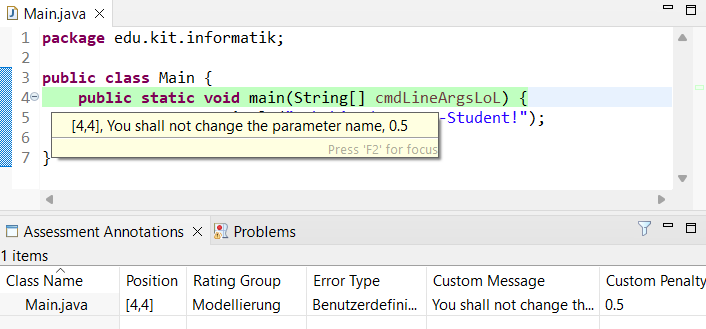
\includegraphics[scale=0.38]{logos/gradingedition_annotation.png}
            \end{center}
        \end{column}
    \end{columns}
\end{frame}

\section{Ansatz}
\subsection{Vorgehen}
\begin{frame}{Ansatz}
	\begin{itemize}
		\item Gegeben: 42 Bewertungsrichtlinien für `Programmieren`          
            \item Aufgabe: Automatisierung durch Tests
            \pause
            \item 2 Fragestellungen: 
            \begin{itemize}
                \item Welche Tools gibt es?
                \item Welche Richtlinien können automatisiert werden?
            \end{itemize}
            \item Tools
            \begin{itemize}
                \item SonarQube $\rightarrow$ 650 Regeln
                \item PMD $\rightarrow$ 325 Regeln
                \item etc.
            \end{itemize}
            \pause
            \item PMD + SonarQube als Quelle
            \item Abbilden der existierenden Regeln zu den eigenen Bewertungsrichtlinien von `Programmieren`
	\end{itemize}
\end{frame}

\begin{frame}{Einbettung}
    \begin{center}
        \vspace{-1cm}
        \hspace{-0.6cm}
        \includesvg[scale=0.75]{logos/workflow_horizontal.svg}
    \end{center}    
\end{frame}

\begin{frame}{Einbettung}
    \begin{center}
        \vspace{-0.85cm}
        \hspace{-0.35cm}
        \includesvg[scale=0.75]{logos/workflow_horizontal_future.svg}
    \end{center}    
\end{frame}

\begin{frame}[fragile]{Ansatz}
    \begin{columns}
\begin{column}{0.7\textwidth}
\hspace{-0.5cm}
\vspace{-0.3cm}
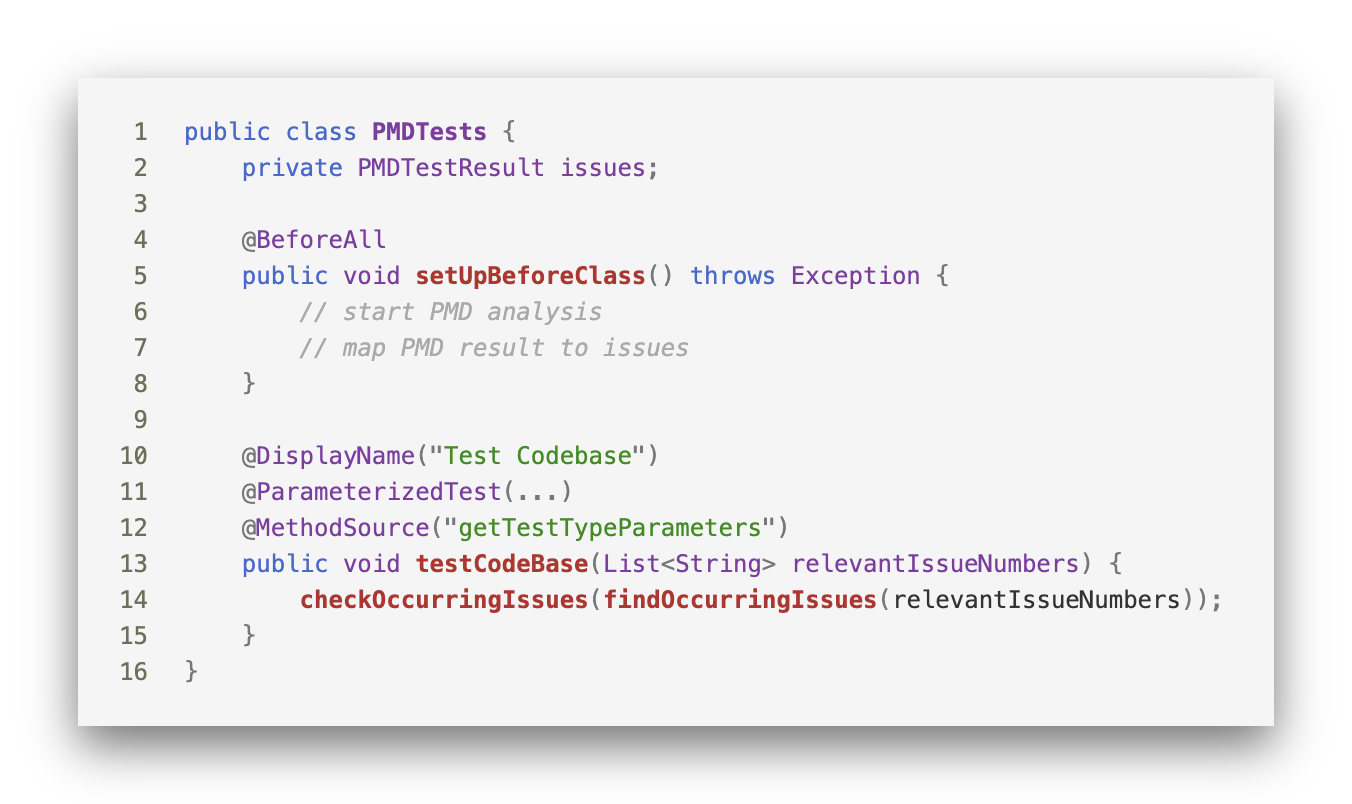
\includegraphics[scale=0.23]{logos/PMDTestCase.png}
% \begin{itemize}
%         \item PMD + SonarQube: Tests schreiben
%     \end{itemize}
   % \begin{lstlisting}
   %      public class PMDTests {
   %          private PMDTestResult issues;

   %          @BeforeAll
   %          public void setUpBeforeClass() throws Exception {
   %              // start PMD analysis
   %              // map PMD result to issues
   %          }

   %          @DisplayName("Test Codebase")
   %          @ParameterizedTest(...)
   %          @MethodSource("getTestTypeParameters")
   %          public void testCodeBase(List<String> relevantIssueNumbers) {
   %              checkOccurringIssues(findOccurringIssues(relevantIssueNumbers));
   %          }
   %      }  
   %  \end{lstlisting}
\end{column}
\begin{column}{0.3\textwidth}  %%<--- here
    \begin{center}
    \hspace{-1cm}
     \includesvg[scale=0.65]{logos/PMDResult_reduced.svg}
     \end{center}
\end{column}
\end{columns}
    
\end{frame}

\subsection{PMD + SonarQube}

\begin{frame}{Raw Type (Nr. 3740)}
    \begin{columns}
        \begin{column}{0.58\textwidth}
            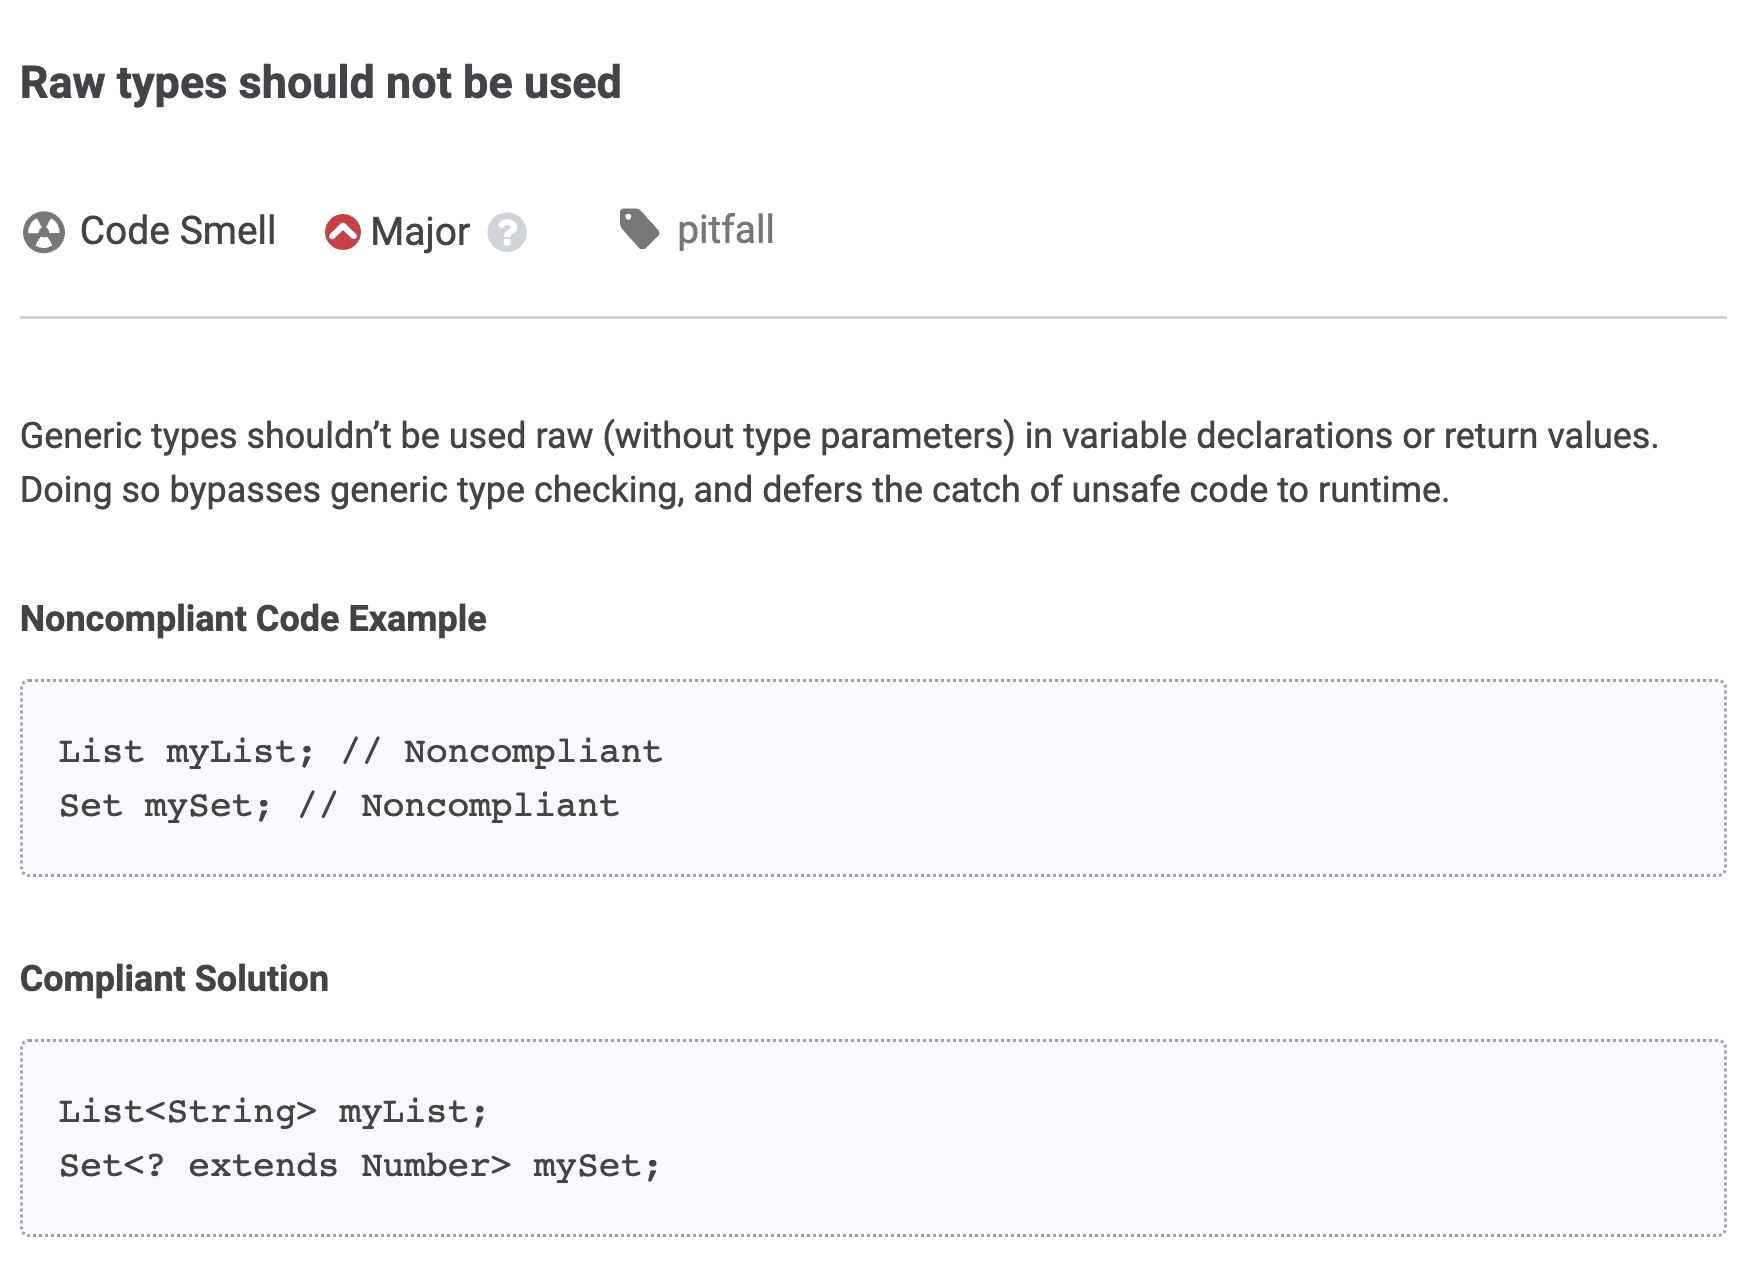
\includegraphics[scale=0.27]{logos/RawTypeSonarQube.png}
        \end{column}
        \begin{column}{0.38\textwidth}
            \begin{figure}
                \hspace{-1.25cm}
                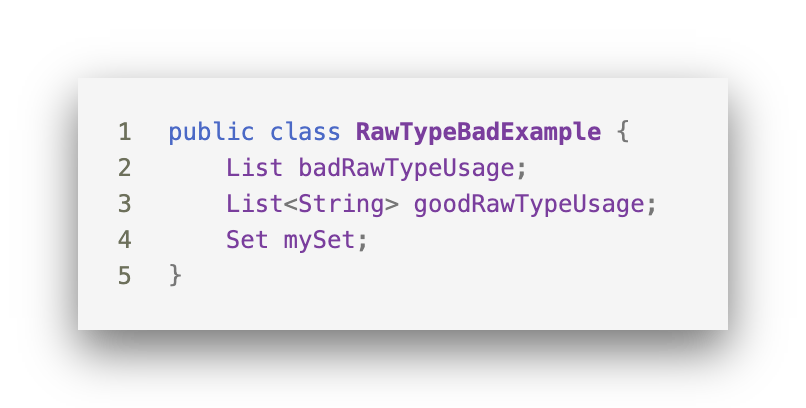
\includegraphics[scale=0.25]{logos/RawTypeBadExample.png}
            \end{figure}
        \end{column}
    \end{columns}
\end{frame}

\begin{frame}{Verknüpfen existierender Regeln}
	\begin{itemize}
		\item Es matchen von PMD + SonarQube zusammen 7 Regeln
            \begin{itemize}
                \item \textit{Utility class}
                \item \textit{Empty constructor}
                \item \textit{Empty block}
                \item \textit{Unused element}
                \item \textit{Final modifier}
                \item \textit{Raw type}
                \item \textit{Class instead of interface}
            \end{itemize}
            \item zudem (+4) Regeln, die Teilmenge der eigentlichen Richtlinie 
            abdecken
            \begin{itemize}
                \item \textit{Code duplication}
                \item \textit{Exceptions for control flow (empty catch block)}
                \item \textit{Hardcoded logic}
                \item \textit{Wrong loop type}
            \end{itemize}
	\end{itemize}
\end{frame}

\section{Erweiterungen}
\begin{frame}{Erweiterungen}
	\begin{itemize}
		\item PMD + SonarQube als Quelle reicht nicht aus
            \item PMD bietet Möglichkeit, eigene Regeln zu erstellen
	\end{itemize}
\end{frame}

\begin{frame}[fragile]{Eigene Regeln}
\vspace{-0.5cm}
\hspace{-0.7cm}
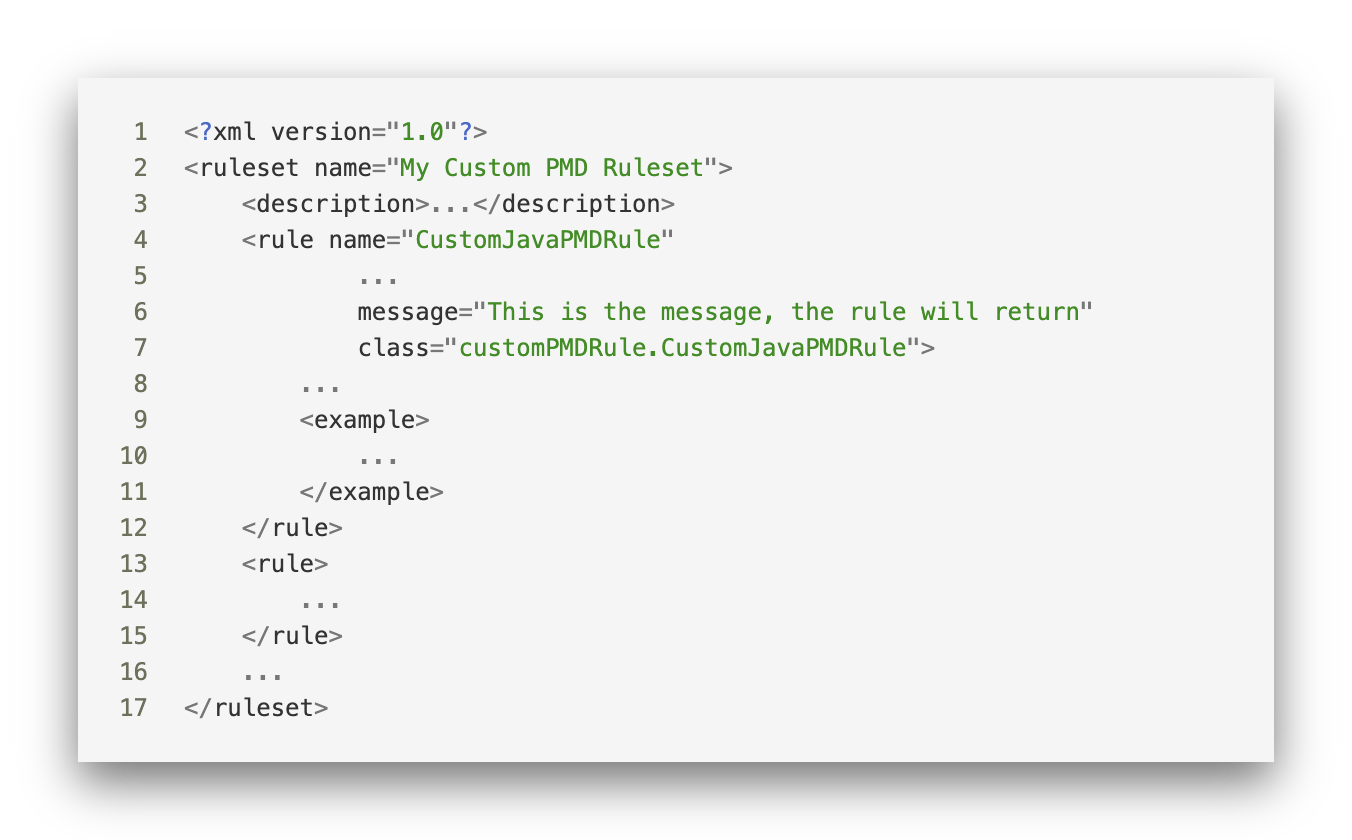
\includegraphics[scale=0.24]{logos/CustomRulesetXML.png}
    % \begin{lstlisting}
    %     <?xml version="1.0"?>
    %     <ruleset name="My Custom PMD Ruleset">
    %         <description>...</description>
    %         <rule name="CustomJavaPMDRule"
    %               ...
    %               message="This is the message, the rule will return"
    %               class="customPMDRule.CustomJavaPMDRule">
    %             ...
    %             <example>
    %                 ...
    %             </example>
    %         </rule>
    %         <rule>
    %             ...
    %         </rule>
    %         ...
    %     </ruleset>
    % \end{lstlisting}
\end{frame}

\begin{frame}[fragile]{Eigene Regeln}
    \vspace{-0.5cm}
    \hspace{-0.7cm}
    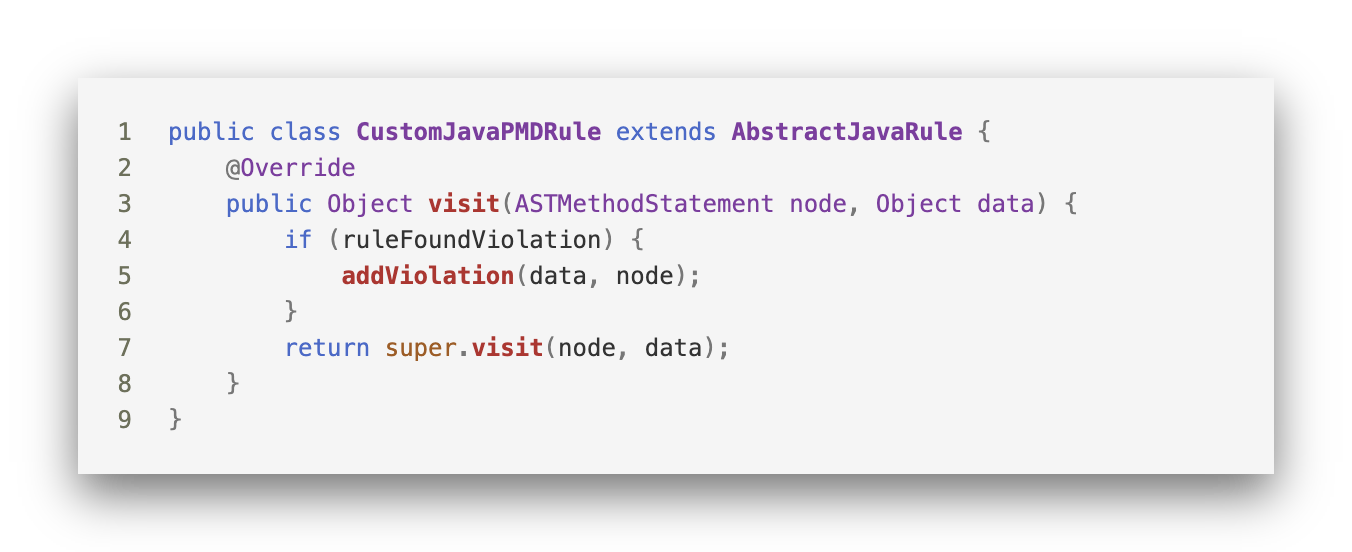
\includegraphics[scale=0.25]{logos/CustomRuleJava.png}
    % \begin{lstlisting}
    %     public class CustomJavaPMDRule extends AbstractJavaRule {
    %         @Override
    %         public Object visit(ASTMethodStatement node, Object data) {
    %             if (ruleFoundViolation) {
    %                 addViolation(data, node);
    %             }
    %             return super.visit(node, data);
    %         }
    %     }
    % \end{lstlisting}
\end{frame}

\begin{frame}{Eigene Regeln}
    \begin{itemize}
        \item \textit{Assert vs If}
        \item \textit{Class of constants}
        \item \textit{Line separator}
        \item \textit{Public enum in class or interface}
        \item \textit{Try catch block size}
    \end{itemize}
\end{frame}

\begin{frame}[fragile]{Eigene Regeln: Public enum in class or interface}
    \vspace{-0.5cm}
    \hspace{-0.7cm}
    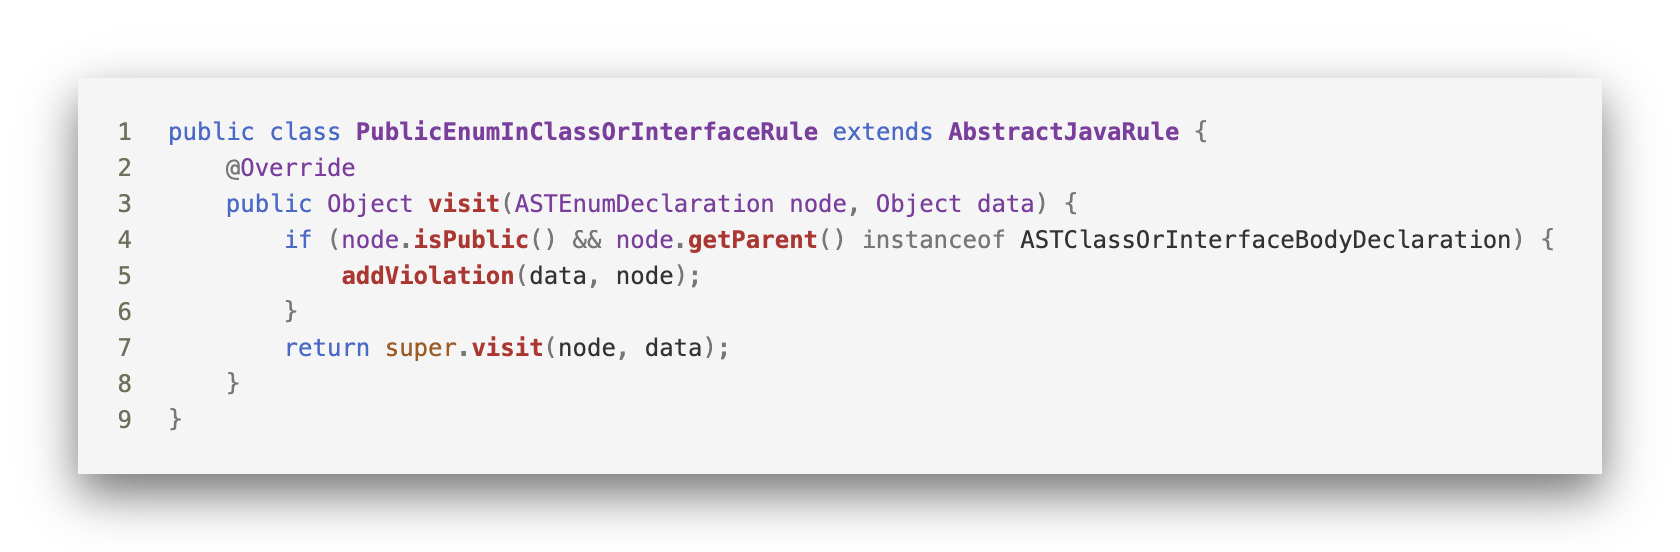
\includegraphics[scale=0.23]{logos/CustomRulePublicEnumInClassOrInterface.png}
    % \begin{lstlisting}
    %     public class PublicEnumInClassOrInterfaceRule extends AbstractJavaRule {
    %         @Override
    %         public Object visit(ASTEnumDeclaration node, Object data) {
    %             if (node.isPublic() && node.getParent() instanceof ASTClassOrInterfaceBodyDeclaration) {
    %                 addViolation(data, node);
    %             }
    %             return super.visit(node, data);
    %         }
    %     }
    % \end{lstlisting}
\end{frame}

\section{Ergebnis}
\begin{frame}{Ergebnis}
	\begin{itemize}
            \item Automatisierung von 16 Bewertungsrichtlinien
            \item Beim Korrigieren:
            \begin{itemize}
                \item Zeitersparnis
                \item Höhere Genauigkeit
                \item Fairness
            \end{itemize}
            \item Future work: 
            \begin{itemize}
                \item Integration in Artemis
                \begin{itemize}
                    \item Studenten haben vor Korrektur auch Einsicht darauf
                \end{itemize}
                \item Weitere 'custom rules' entwickeln!
            \end{itemize}
	\end{itemize}
\end{frame}

\appendix
\beginbackup

\begin{frame}[fragile]{Eigene Regeln: AssertVsIF}
    \vspace{-0.5cm}
    \hspace{-0.7cm}
    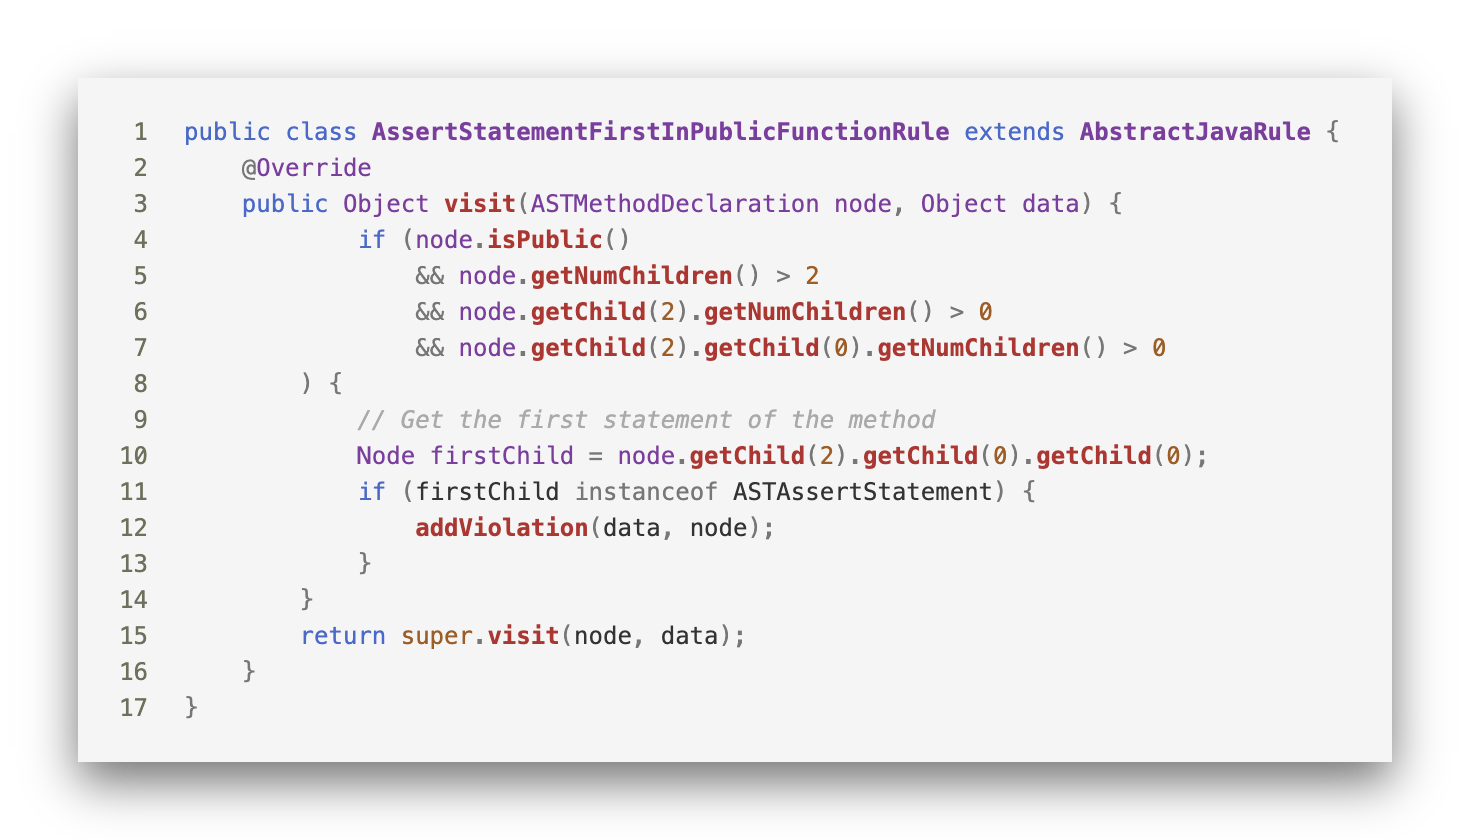
\includegraphics[scale=0.23]{logos/CustomRuleAssertVsIf.png}
    % \begin{lstlisting}
    %     public class AssertStatementFirstInPublicFunctionRule extends AbstractJavaRule {
    %         @Override
    %         public Object visit(ASTMethodDeclaration node, Object data) {
    %              if (node.isPublic()
    %                     && node.getNumChildren() > 2
    %                     && node.getChild(2).getNumChildren() > 0
    %                     && node.getChild(2).getChild(0).getNumChildren() > 0
    %             ) {
    %                 // Get the first statement of the method
    %                 Node firstChild = node.getChild(2).getChild(0).getChild(0);
    %                 if (firstChild instanceof ASTAssertStatement) {
    %                     addViolation(data, node);
    %                 }
    %             }
    %             return super.visit(node, data);
    %         }
    %     }
    % \end{lstlisting}
\end{frame}

\begin{frame}[fragile]{Eigene Regeln: ClassOfConstants}
    \vspace{-0.5cm}
    \hspace{-0.7cm}
    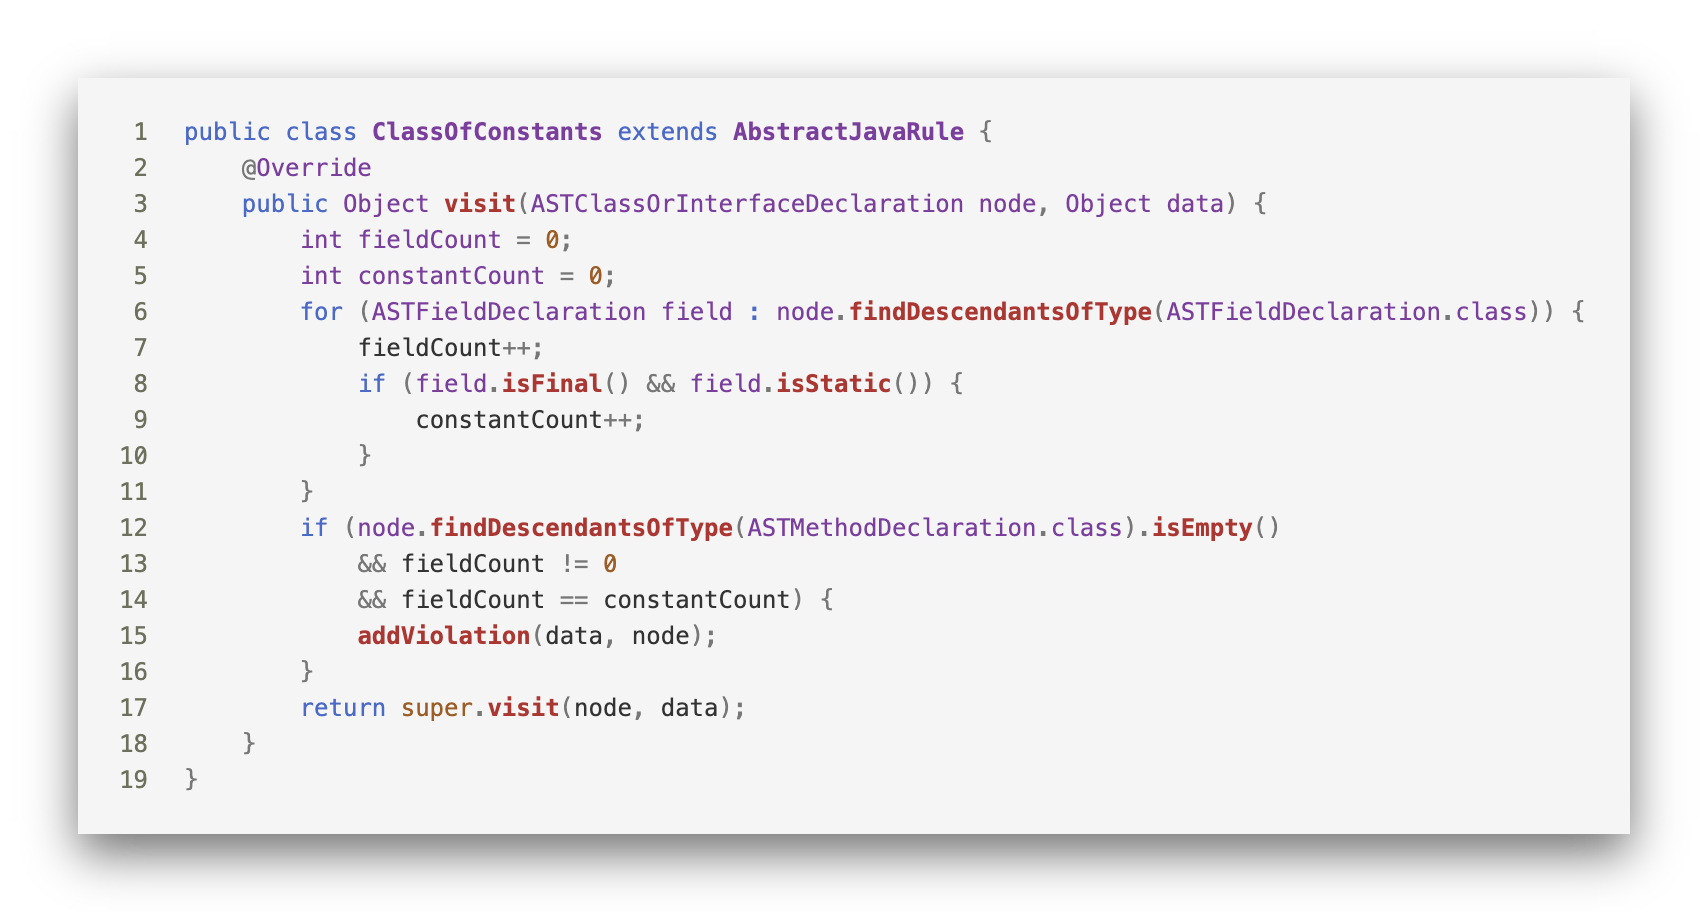
\includegraphics[scale=0.22]{logos/CustomRuleClassOfConstants.png}
    % \begin{lstlisting}
    %     public class ClassOfConstants extends AbstractJavaRule {
    %         @Override
    %         public Object visit(ASTClassOrInterfaceDeclaration node, Object data) {
    %             int fieldCount = 0;
    %             int constantCount = 0;
    %             for (ASTFieldDeclaration field : node.findDescendantsOfType(ASTFieldDeclaration.class)) {
    %                 fieldCount++;
    %                 if (field.isFinal() && field.isStatic()) {
    %                     constantCount++;
    %                 }
    %             }
    %             if (node.findDescendantsOfType(ASTMethodDeclaration.class).isEmpty() 
    %                 && fieldCount != 0 
    %                 && fieldCount == constantCount) {
    %                 addViolation(data, node);
    %             }
    %             return super.visit(node, data);
    %         }
    %     }
    % \end{lstlisting}
\end{frame}

\begin{frame}[fragile]{Eigene Regeln: LineBreakRule}
    \vspace{-0.5cm}
    \hspace{-0.7cm}
    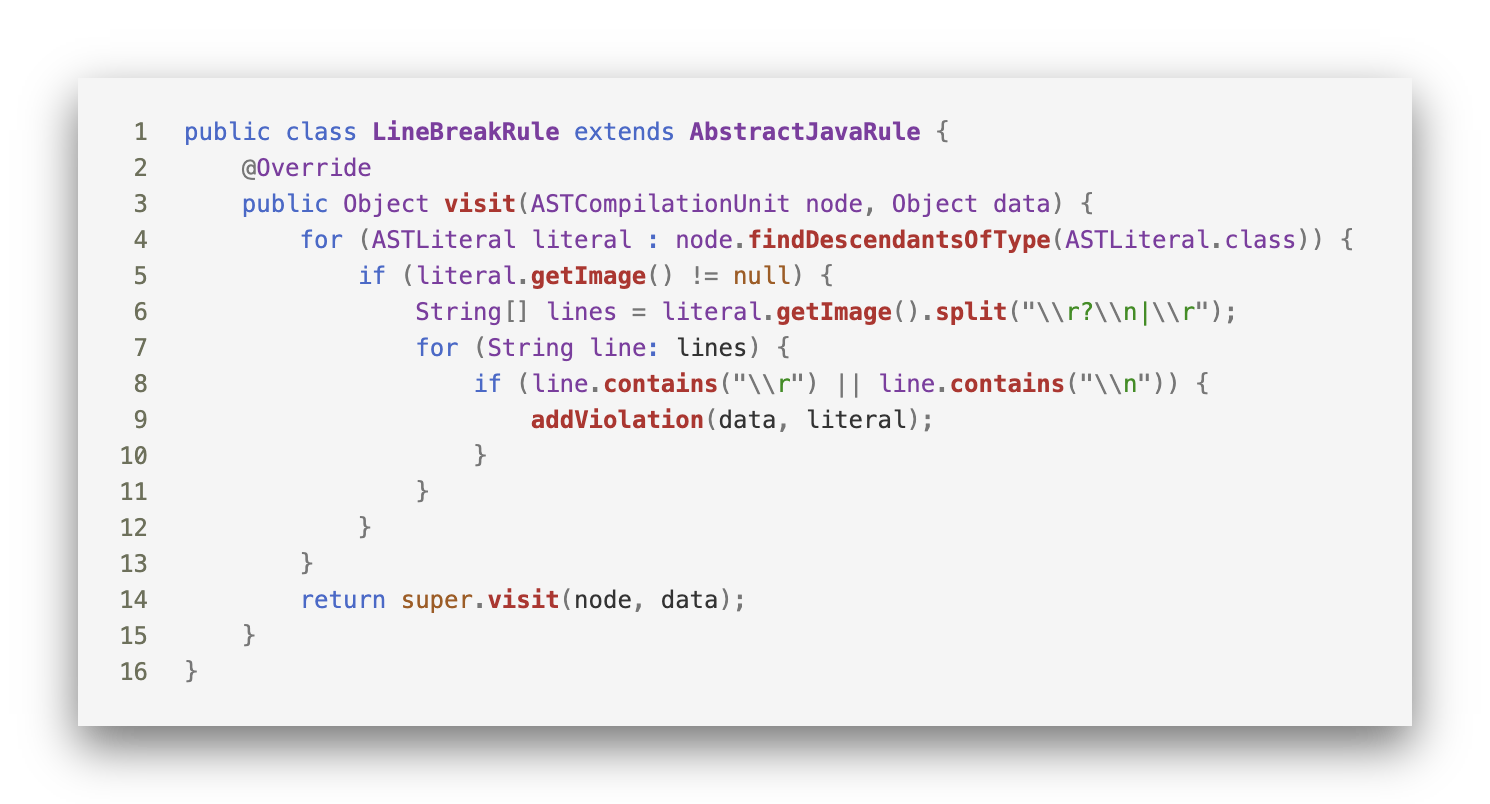
\includegraphics[scale=0.23]{logos/CustomRuleLineBreakRule.png}
    % \begin{lstlisting}
    %     public class LineBreakRule extends AbstractJavaRule {
    %         @Override
    %         public Object visit(ASTCompilationUnit node, Object data) {
    %             for (ASTLiteral literal : node.findDescendantsOfType(ASTLiteral.class)) {
    %                 if (literal.getImage() != null) {
    %                     String[] lines = literal.getImage().split("\\r?\\n|\\r");
    %                     for (String line: lines) {
    %                         if (line.contains("\\r") || line.contains("\\n")) {
    %                             addViolation(data, literal);
    %                         }
    %                     }
    %                 }
    %             }
    %             return super.visit(node, data);
    %         }
    %     }

    % \end{lstlisting}
\end{frame}

\begin{frame}[fragile]{Eigene Regeln: PublicEnumInClassOrInterface}
    \vspace{-0.5cm}
    \hspace{-0.7cm}
    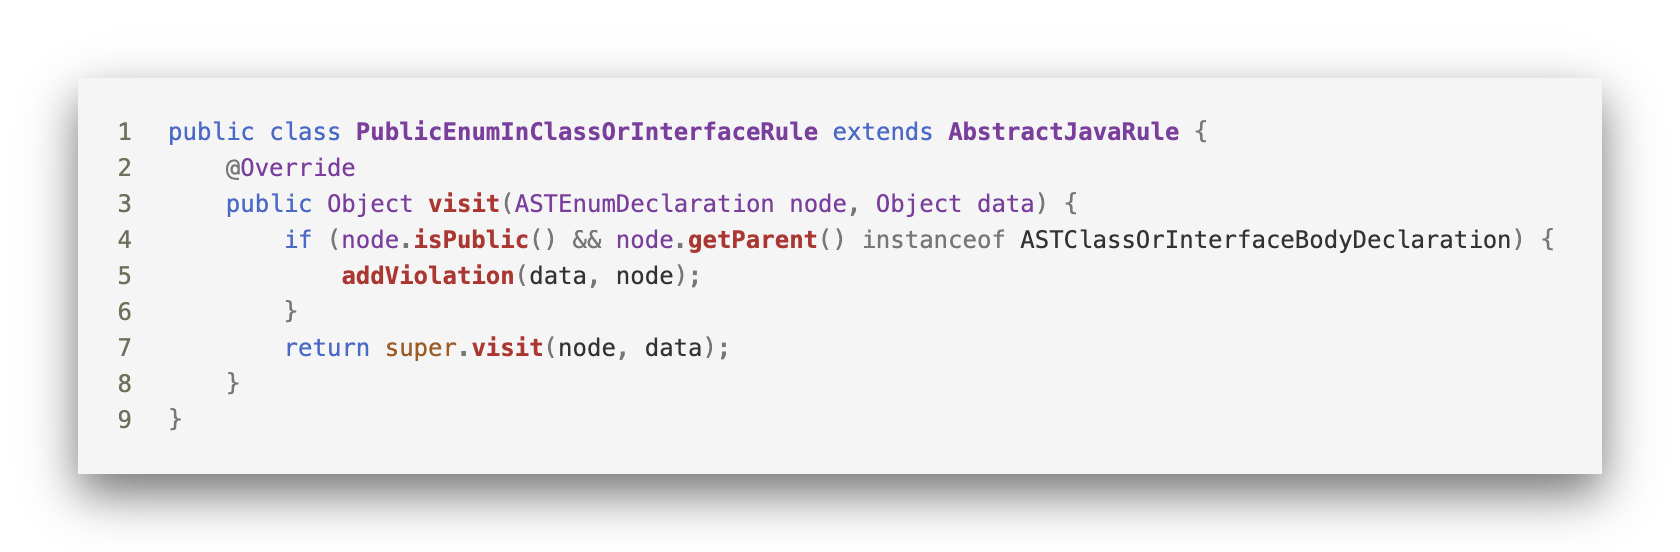
\includegraphics[scale=0.23]{logos/CustomRulePublicEnumInClassOrInterface.png}
    % \begin{lstlisting}
    %     public class PublicEnumInClassOrInterfaceRule extends AbstractJavaRule {
    %         @Override
    %         public Object visit(ASTEnumDeclaration node, Object data) {
    %             if (node.isPublic() && node.getParent() instanceof ASTClassOrInterfaceBodyDeclaration) {
    %                 addViolation(data, node);
    %             }
    %             return super.visit(node, data);
    %         }
    %     }
    % \end{lstlisting}
\end{frame}

\begin{frame}[fragile]{Eigene Regeln: TryCatchBlockSize}
    \vspace{-0.5cm}
    \hspace{-0.7cm}
    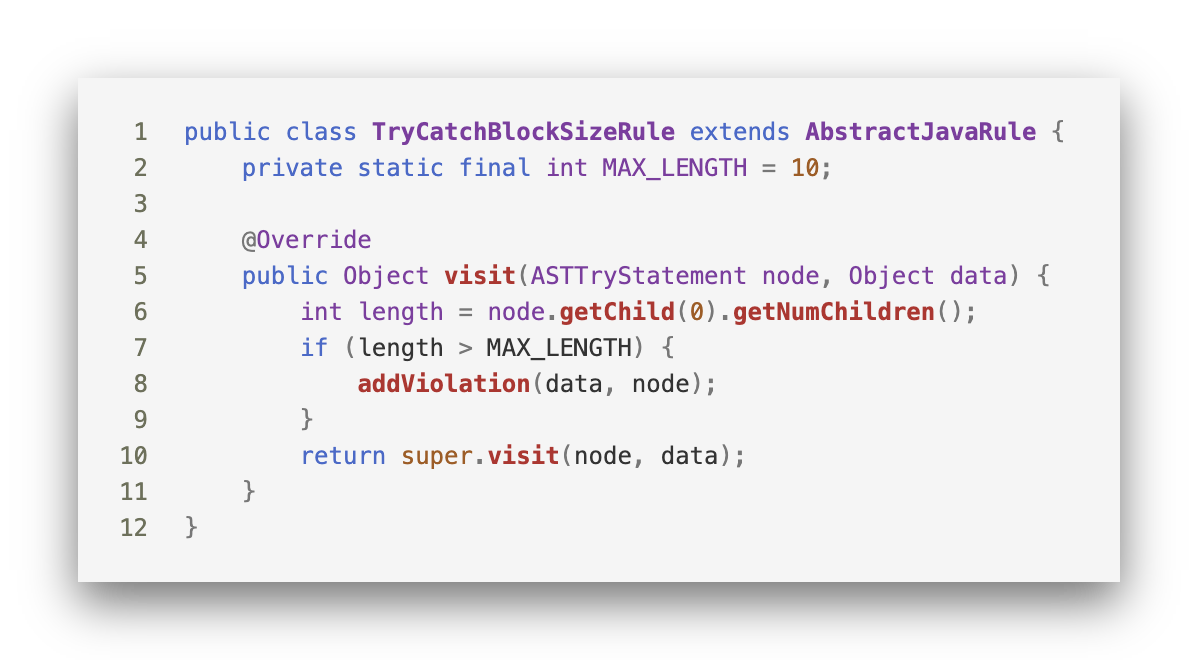
\includegraphics[scale=0.24]{logos/CustomRuleTryCatch.png}
    % \begin{lstlisting}
    %     public class TryCatchBlockSizeRule extends AbstractJavaRule {
    %         private static final int MAX_LENGTH = 10;
        
    %         @Override
    %         public Object visit(ASTTryStatement node, Object data) {
    %             int length = node.getChild(0).getNumChildren();
    %             if (length > MAX_LENGTH) {
    %                 addViolation(data, node);
    %             }
    %             return super.visit(node, data);
    %         }
    %     }
    % \end{lstlisting}
\end{frame}

\begin{frame}[fragile]{Parameterized Test: getTestTypeParameters}
    \vspace{-0.5cm}
    \hspace{-0.7cm}
    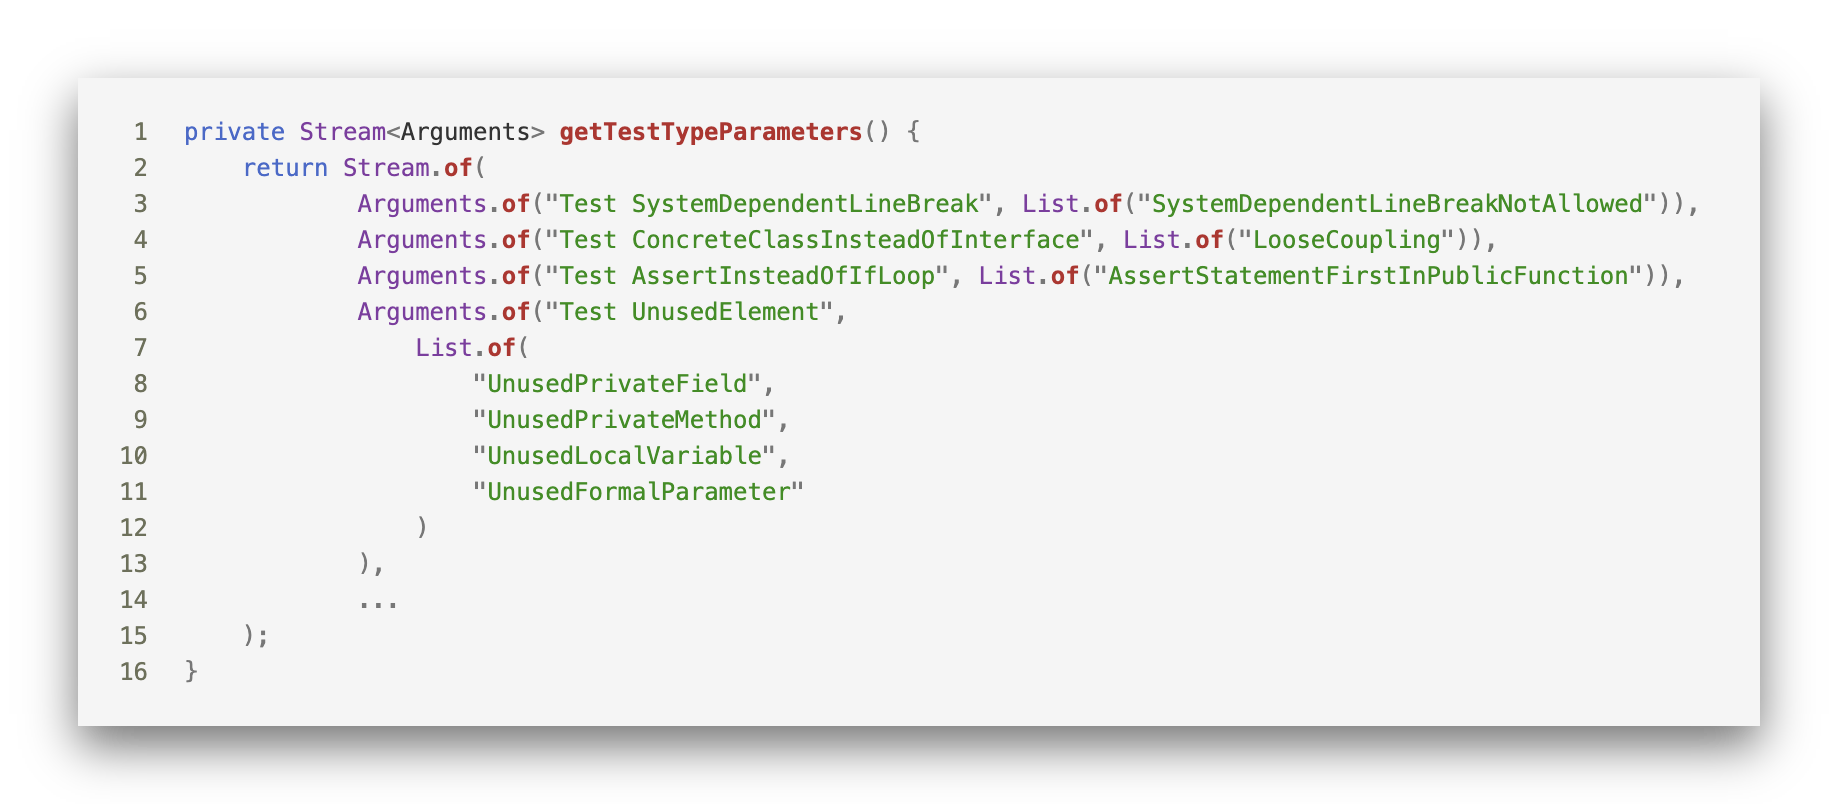
\includegraphics[scale=0.23]{logos/CodeGetTestTypeParameters.png}
    % \begin{lstlisting}
    %     private Stream<Arguments> getTestTypeParameters() {
    %         return Stream.of(
    %                 Arguments.of("Test SystemDependentLineBreak", List.of("SystemDependentLineBreakNotAllowed")),
    %                 Arguments.of("Test ConcreteClassInsteadOfInterface", List.of("LooseCoupling")),
    %                 Arguments.of("Test AssertInsteadOfIfLoop", List.of("AssertStatementFirstInPublicFunction")),
    %                 Arguments.of("Test UnusedElement",
    %                     List.of(
    %                         "UnusedPrivateField", 
    %                         "UnusedPrivateMethod", 
    %                         "UnusedLocalVariable", 
    %                         "UnusedFormalParameter"
    %                     )
    %                 ),
    %                 ...
    %         );
    %     }
    % \end{lstlisting}
\end{frame}

\begin{frame}[fragile]{PMD: BeforeAll}
    \vspace{-0.5cm}
    \hspace{-0.7cm}
    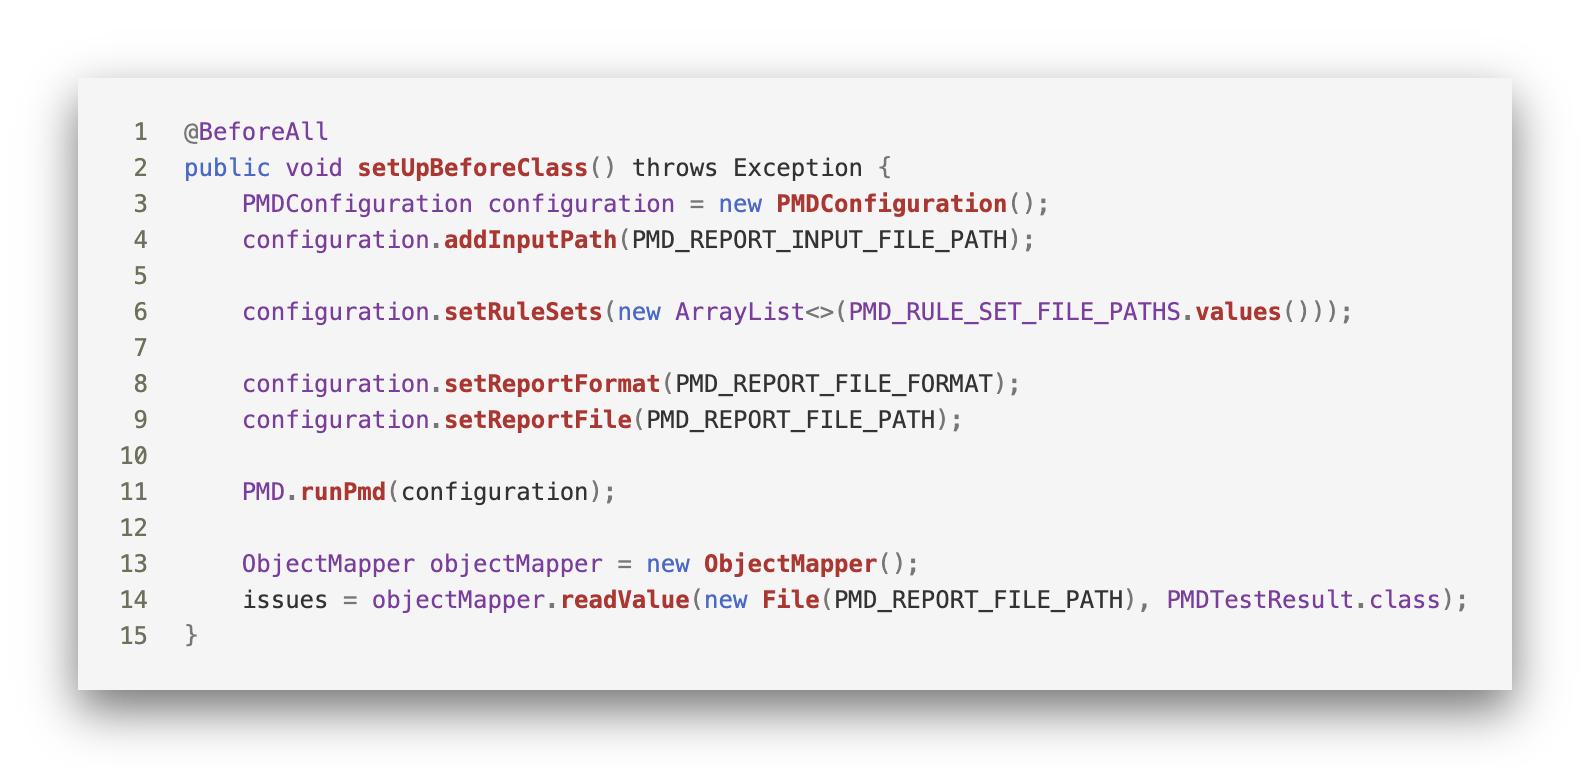
\includegraphics[scale=0.23]{logos/CodeTestBeforeAll.png}
    % \begin{lstlisting}
    %     @BeforeAll
    %     public void setUpBeforeClass() throws Exception {
    %         PMDConfiguration configuration = new PMDConfiguration();
    %         configuration.addInputPath(PMD_REPORT_INPUT_FILE_PATH);
    
    %         configuration.setRuleSets(new ArrayList<>(PMD_RULE_SET_FILE_PATHS.values()));
    
    %         configuration.setReportFormat(PMD_REPORT_FILE_FORMAT);
    %         configuration.setReportFile(PMD_REPORT_FILE_PATH);
    
    %         PMD.runPmd(configuration);
    
    %         ObjectMapper objectMapper = new ObjectMapper();
    %         issues = objectMapper.readValue(new File(PMD_REPORT_FILE_PATH), PMDTestResult.class);
    %     }
    % \end{lstlisting}
\end{frame}

\begin{frame}{Literatur}
\begin{exampleblock}{Titelbilder Quelle:}
    Das Titelbild wurde aus den 2 Bildern von (\cite{pmdLogo}) und  (\cite{sonarqubeLogo}) zusammengesetzt.
\end{exampleblock}
\begin{exampleblock} {RawType Quelle:}
    Der Screenshot stammt von der offiziellen SonarQube Documentation Website (\cite{rawTypeSQLink}).
    
\end{exampleblock}
\end{frame}

\begin{frame}{Literatur}
    \printbibliography
\end{frame}

\section{Farben}
\backupend

\end{document}